\documentclass[12pt]{article}
\usepackage[UTF8]{ctex}  % 中文支持

\usepackage[utf8]{inputenc}
\usepackage{amsmath}
\usepackage{amssymb}
\usepackage{geometry}
\usepackage{graphicx}
\usepackage{amsmath, amssymb}
\usepackage{geometry}
\usepackage{tikz}
\usetikzlibrary{intersections}

\geometry{a4paper, margin=1in}

% \title{Homework 1206}
% \author{Liu}
% \date{\today}
\begin{document}


\section*{差不变规律}
如图，正方形 $ABCD$ 的边长为 $6\,\mathrm{cm}$，$CF=8\,\mathrm{cm}$，求阴影部分甲比乙的面积大多少？
\begin{center}
    \begin{tikzpicture}[scale=0.6]
        % 正方形 ABCD
        \coordinate (B) at (0,0);
        \coordinate (C) at (6,0);
        \coordinate (D) at (6,6);
        \coordinate (A) at (0,6);
        \draw (A) -- (B) -- (C) -- (D) -- cycle;
        \node[ left] at (A) {A};
        \node[left] at (B) {B};
        \node[below] at (C) {C};
        \node[right] at (D) {D};
        % 点 E 是 AB 中点 
        \coordinate (E) at (6,3.428);
        \node[below left] at (E) {E};
        % 点 F 在 CD 延长线上
        \coordinate (F) at (14,0);
        \node[right] at (F) {F};
        %  辅助线 
        \draw (C) -- (E);
        \draw (A) -- (F);
        \draw (E) -- (F);
        %  标注边长
        %   \node at (3,-0.5) {$6\,\mathrm{cm}$}; \node at (6.5,10) {$8\,\mathrm{cm}$}; % 阴影区域甲（CEF） 
        \fill[gray!30] (C) -- (E) -- (F) -- cycle; \node at (9,1) {甲}; % 阴影区域乙（ABE） 
        \fill[gray!50] (A) -- (D) -- (E) -- cycle; \node at (5,5) {乙};
         \draw (C) -- (D);
         \draw (C) -- (F);
         \draw (A) -- (F);
    \end{tikzpicture}
\end{center}

如图，平行四边形 $ABCD$ 的边 $BC$ 长 $12$ 厘米，直角三角形 $BCE$ 的直角边 $CE$ 长 $10$ 厘米，已知阴影部分的面积比三角形 $EFG$ 的面积大 $18$ 平方厘米，求 $EF$ 的长。
\begin{center}
    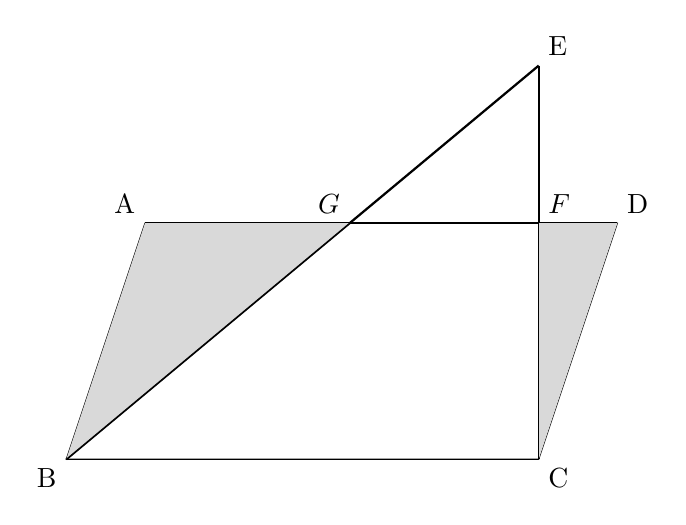
\begin{tikzpicture}[scale=0.5] % 点坐标 
        \coordinate (B) at (0,0);
        \coordinate (C) at (12,0);
        \coordinate (D) at (14,6);
        \coordinate (A) at (2,6);
        \coordinate (E) at (12,10);
        \coordinate (F) at (6,8);
        \coordinate (G) at (10,4); % 平行四边形 ABCD 
        \draw (A) -- (B) -- (C) -- (D) -- cycle;
        \draw[name path=lineA, thick] (B) -- (E);
        \draw[name path=lineB, thick] (A) -- (D);
        % 计算交点 1
        \path [name intersections={of=lineA and lineB, by=G}];
        % 标记交点
        \filldraw (G)  node[above left] {$G$};
        \draw[name path=lineA, thick] (E) -- (C);

        % 计算交点 1
        \path [name intersections={of=lineA and lineB, by=F}];
        % 标记交点
        \filldraw (F)  node[above right] {$F$};
        \node[above left] at (A) {A};
        \node[below left] at (B) {B};
        \node[below right] at (C) {C};
        \node[above right] at (D) {D}; % 三角形 BCE 
        % \draw (B) -- (E) -- (C);
        \node[above right] at (E) {E}; % 三角形 EFG 
        % \draw (E) -- (F) -- (G) -- cycle;
        \fill[gray!30] (C) -- (F) -- (D) -- cycle;
        \fill[gray!30] (A) -- (B) -- (G) -- cycle;
        \draw (B) --(G);
        \draw (F) --(C);
        % \fill[gray!30] (A) -- (B) -- (C) -- (E) -- cycle; % 标注边长 
        % \draw[<->] (B)++(0,-1) --++ (12,0) node[midway, below] {$12\,\mathrm{cm}$};
        % \draw[<->] (C)++(0,0) --++ (0,10) node[midway, right] {$10\,\mathrm{cm}$};

    \end{tikzpicture}
\end{center}
\end{document}